\documentclass{beamer}

\usepackage{beamerthemesplit}
\usetheme{boxes} 
\setbeamertemplate{items}[default] 
\setbeamertemplate{blocks}[rounded]
\setbeamertemplate{navigation symbols}{} 
 
% Math macros
\newcommand{\cD}{{\mathcal D}}
\newcommand{\cF}{{\mathcal F}}
\newcommand{\todo}[1]{{\color{red}{TO DO: \sc #1}}}

\newcommand{\reals}{\mathbb{R}}
\newcommand{\integers}{\mathbb{Z}}
\newcommand{\naturals}{\mathbb{N}}
\newcommand{\rationals}{\mathbb{Q}}

\newcommand{\ind}[1]{1{\{#1\}}} % Indicator function
\newcommand{\pr}{\mathbb{P}} % Generic probability
\newcommand{\ex}{\mathbb{E}} % Generic expectation
\newcommand{\var}{\textrm{Var}}
\newcommand{\cov}{\textrm{Cov}}

\newcommand{\normal}{N} % for normal distribution (can probably skip this)
\newcommand{\eps}{\varepsilon}
\newcommand\independent{\protect\mathpalette{\protect\independenT}{\perp}}
\def\independenT#1#2{\mathrel{\rlap{$#1#2$}\mkern2mu{#1#2}}}

\newcommand{\convd}{\stackrel{d}{\longrightarrow}} % convergence in distribution/law/measure
\newcommand{\convp}{\stackrel{P}{\longrightarrow}} % convergence in probability
\newcommand{\convas}{\stackrel{\textrm{a.s.}}{\longrightarrow}} % convergence almost surely

\newcommand{\eqd}{\stackrel{d}{=}} % equal in distribution/law/measure
\newcommand{\argmax}{\arg\!\max}
\newcommand{\argmin}{\arg\!\min}
 \newcommand{\bit}{\begin{itemize}}
 \newcommand{\eit}{\end{itemize}}
 
 
%%%%%%%%%%%%%%%%%%%%%%%%%%%%%%%%%%%%%%%%%%%%%

\title{A review of ``On the Failure of the Bootstrap for Matching Estimators'' (Abadie and Imbens; 2008)}
\author{Andrew Do, Kellie Ottoboni, Simon Walter}
\date{April 8, 2016}

\begin{document}

\frame{\titlepage}

\section[Outline]{}
\frame{\tableofcontents}

\section{Introduction}

\frame{
\frametitle{Problem}

\bit
\item Matching is sometimes done to control for pretreatment covariates in observational studies
\item Matching estimators are nonlinear functions of the data and do not follow any nice known distribution
\item \textbf{Problem:} how do you find standard errors for matching estimators?
\item Two common ways: asymptotic approximations and resampling methods
\eit
}

\frame
{
  \frametitle{The bootstrap}
\begin{figure}  
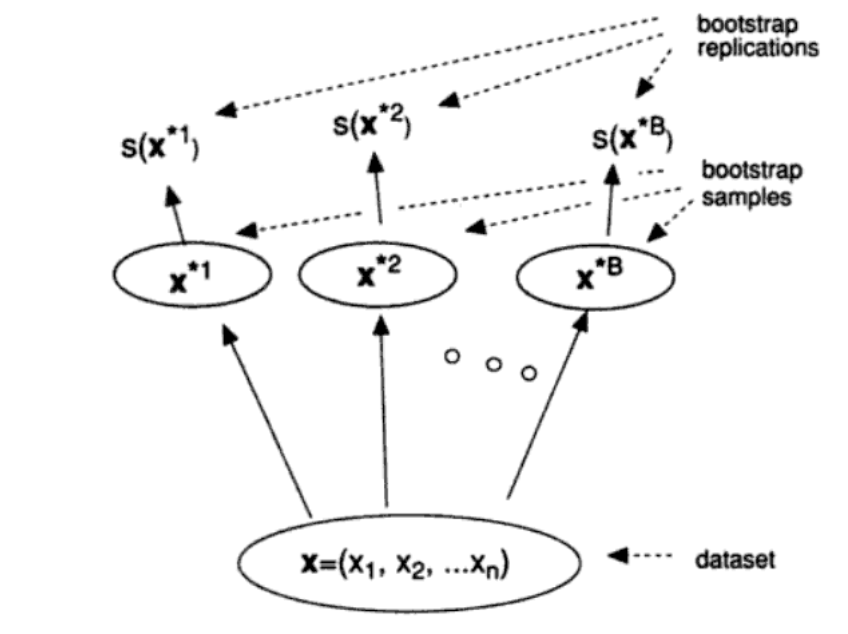
\includegraphics[width = 0.8\textwidth]{fig/scheme.png}
\end{figure}
Sample with replacement from the observed data, pretending it is the population, to approximate the distribution of the statistic
\todo{Anyone know of a better graphic?}
\todo{cite Efron and Tibshirani book from which I screenshotted this}
}





\frame{
\frametitle{On the failure of the bootstrap}

The bootstrap estimate of the variance of the matching estimator $\hat{\tau}$ is given by
$$\hat{V}^B = \frac{1}{B} \sum_{b=1}^B \left( \hat{\tau}_b - \hat{\tau} \right)^2$$

\textbf{Abadie and Imbens show that $\hat{V}^B$ is not generally valid for matching estimators.} \\
\vspace{10pt}
They focus on the case of one-to-one matching on a single continuous covariate.
}


\section{Abadie and Imbens (2008)}

\subsection{Notation and Assumptions}

\frame{
\frametitle{Notation and Assumptions}
\begin{itemize}
\item Suppose we have a random sample of $N_0$ units from the control population and a random sample of $N_1$ units from the treated population, with $N = N_0 + N_1$
\item Each unit has a pair of potential outcomes, $Y_i(0)$ and $Y_i(1)$, under the control and active treatments
\item Let $W_i$ indicate treatment: we observe $Y_i = W_i Y_i(1) + (1-W_i) Y_i(0)$
\item In addition to the outcome, we observe a (scalar) covariate $X_i$ for each individual
\end{itemize}
We're interested in the \textbf{average treatment effect for the treated} (ATT):

$$\tau = \ex(Y_i(1) - Y_i(0) \mid W_i = 1)$$
}


\frame{
\frametitle{Notation and Assumptions}

We make the usual assumptions for matching:

\begin{itemize}
\item Unconfoundedness: For almost all $x$,
$$(Y_i(0), Y_i(1)) \independent W_i \mid X_i = x \text{  almost surely}$$
\item Overlap: For some $0 < c < 1$ and almost all $x$,
$$c \leq \pr(W_i = 1 \mid X_i = x) \leq 1-c$$
\end{itemize}
}



\frame{
\frametitle{Notation and Assumptions}
$D_i$ is the distance between the covariate values for observation $i$ and the closest control group match:

$$D_i = \min_{j = 1, \dots, N: W_j = 0} \left\Vert X_i - X_j \right\Vert$$

\vspace{20pt}
$\mathcal{J}(i)$ is the set of closest matches for treated unit $i$. 

\begin{displaymath}
   \mathcal{J}(i) = \left\{
     \begin{array}{lr}
       \{ j \in \{1, \dots, N\} : W_j = 0, \left\Vert X_i - X_j \right\Vert = D_i \} & \text{ if  } W_i = 1\\
       \emptyset & \text{ if  } W_i = 0
     \end{array}
   \right.
\end{displaymath} 

If $X$ is continuous, this set will consist of one unit with probability 1. In bootstrap samples, units may appear more than once.
}


\frame{
\frametitle{Notation and Assumptions}
Estimate the counterfactual for each treated unit as:

$$\hat{Y}_i(0) = \frac{1}{\# \mathcal{J}(i)} \sum_{j \in \mathcal{J}(i)} Y_i$$

The matching estimator of $\tau$ is then

$$\hat{\tau} = \frac{1}{N_1} \sum_{i : W_i = 1} \left(Y_i - \hat{Y}_i(0)\right)$$
}




\frame{
\frametitle{Notation and Assumptions}
An alternative way of writing the estimator is

$$\hat{\tau} = \frac{1}{N_1} \sum_{i=1}^N (W_i - (1-W_i)K_i) Y_i$$

where $K_i$ is the weighted number of times that unit $i$ is used as a match:

\begin{displaymath}
   K_i = \left\{
     \begin{array}{lr}
      0 & \text{ if  } W_i = 1\\
      \sum_{j: W_j=1} \ind{i \in \mathcal{J}(j)} \frac{1}{\#\mathcal{J}(j)} & \text{ if  } W_i = 0
     \end{array}
   \right.
\end{displaymath} 
}



\subsection{The Bootstrap}



\frame{
\frametitle{Bootstrap}
\bit
\item We obtain a \textbf{bootstrap sample} $Z_b$ by taking a random sample with replacement from $Z= (X, W, Y)$. 
\item Let $\hat{\tau}_b = t(Z_b)$ be the matching statistic computed on bootstrap sample $b$.
\item The bootstrap variance of $\hat{\tau}$ is the variance of $\hat{\tau}_b$ conditional on the original data $Z$:

$$V^{B} = \ex\left[ (\hat{\tau}_b - \hat{\tau})^2 \mid Z\right]$$

\item We estimate it by generating $B$ bootstrap samples from $Z$ and taking the following average:

$$\hat{V}^B = \frac{1}{B} \sum_{b=1}^B \left( \hat{\tau}_b - \hat{\tau} \right)^2$$
\eit
}


\frame{
\frametitle{Bootstrap}
\bit
\item The bootstrap works for linear statistics that are consistent and asymptotically normal
\item For nonlinear statistics, the bootstrap requires additional smoothness conditions \todo{cite?}
\item \todo{Abadie and Imbens show that $\hat{\tau}$ is asymptotically normal with ugly variance}
\item Why does the bootstrap fail here? 
\eit


}


\frame{
\frametitle{Bootstrap}
\textbf{Issue:} the bootstrap fails to replicate the distribution of $K_i$, even in large samples.
\vspace{10pt}


Example:
\begin{itemize}
\item Suppose the ratio $N_1/N_0$ is small (i.e. there are many more controls than treated)
\item In the original sample, few controls are used as a match more than once
\item In bootstrap samples, treated units may appear multiple times, creating situations where $\pr(K_{b,i} > 1) > \pr(K_i > 1)$ \todo{is this technically correct? is there a better way to put this?}
\end{itemize}
}


\section{Simulations} % can change the subsection headings...

\subsection{Example 1} % Andrew results

\subsection{Example 2} % Kellie results


\frame{
\frametitle{Effect of covariate distributions}

\bit
\item Potential outcomes $Y(1)$ and $Y(0)$ defined as before
\item Treatment assigned at random with $\frac{N_1}{N_0} = \alpha = 2$ fixed
\item Change the covariate distributions: $X_i \sim N(0, 1)$ if $W_i = 1$ and $X_i \sim N(\mu, 1)$ if $W_i = 0$.
\item We vary $\mu$ from $0$ to $5$
\item \todo{this slide is ugly}
\eit
}

\frame{
\frametitle{Results}
\begin{figure}[htbp]
\begin{center}
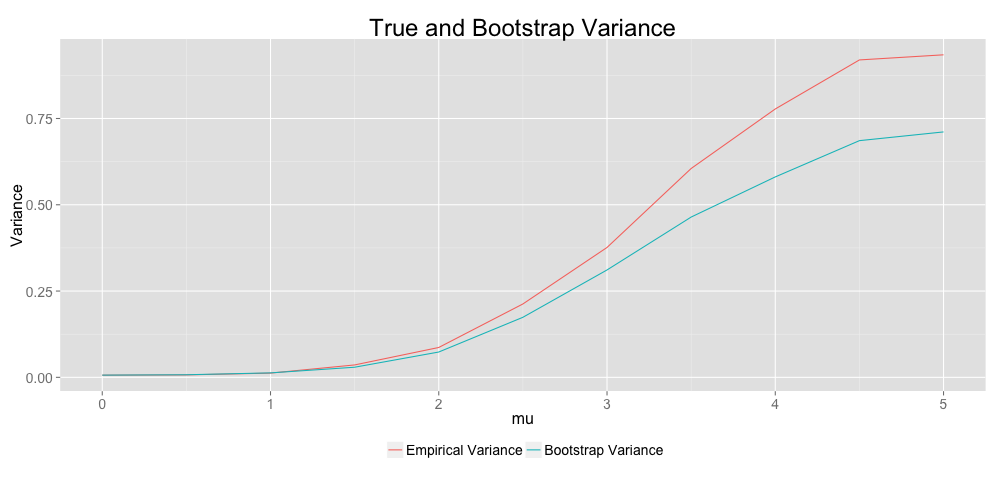
\includegraphics[width = 0.85\textwidth]{fig/KellieSimulationBias.png}
\end{center}
\end{figure}

The bootstrap tends to underestimate the variance of $\hat{\tau}$.  The bias increases as the distance $\mu$ between treatment and control groups increases.
}


\frame{
\frametitle{Results}
\begin{figure}[htbp]
\begin{center}
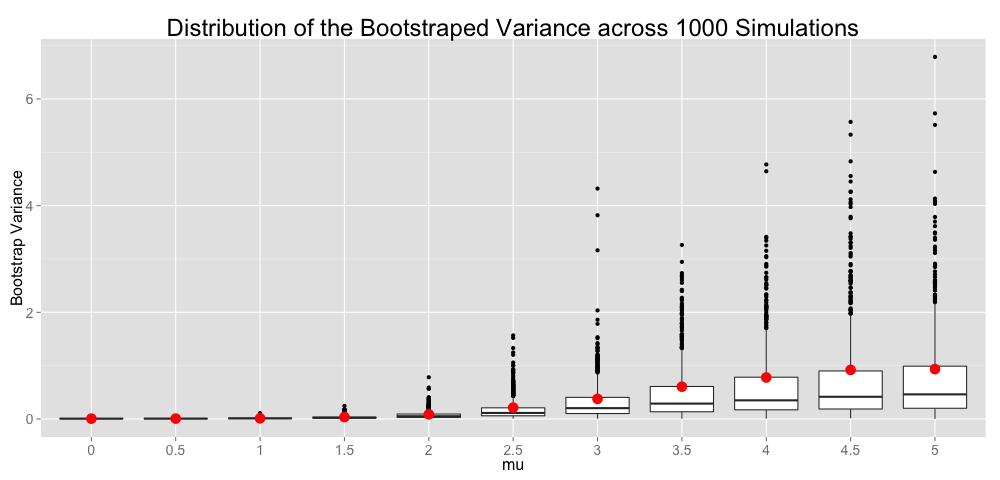
\includegraphics[width = 0.9\textwidth]{fig/KellieSimulationDistr.png}
\end{center}
\end{figure}

Red points indicate the observed variance of the test statistic.  The distribution of bootstrap variances has a long right tail. The skew worsens as $\mu$ grows.

}


\frame{
\frametitle{Placing Abadie and Imbens in the literature}
\bit
%\item There is a widespread but imperfect and outdated intuition that states that Efron's bootstrap consistently estimates the distribution of the statistic  if and only if the statistic is asymptotically normal. 
\item Cs\"{o}rg\H{o} and Mason (1989) established that linear statistics are consistently estimated by the bootstrap if and only if they are asymptotically normal. 

\item \todo{X (198?)} suggests rigorous results for non-linear statistics require in addition to asymptotic normality that the statistic is a smooth function of the data. 
\item Formalizing this requires a notion of smoothness of random quantities called Fr\'{e}chet differentiability, but we will elide it.
\eit
}
\frame{
\frametitle{Placing Abadie and Imbens in the literature}
\bit
\item The revision history of the manuscript  suggests that at least initially Abadie and Imbens were not particularly familiar with this prior work and some vestiges of this position remain.

\item The results of Abadie and Imbens are not surprising and  not novel to specialists familiar with the theoretical work of the 1980s.
\item But it is valuable because it informs practitioners one of the (many) limitations of the vanilla bootstrap. 
%\item For example in the Beran's (1982) example it is not hard to show this is violated:
%\begin{align*}
%\theta(X_1, \ldots, X_n) \Longrightarrow
%N\left[\mu, \frac{1}{n} \var(X))\right] \textrm{\quad   if $E(X) \neq 0$} \\
%\theta(X_1, \ldots, X_n) \Longrightarrow N\left[\mu, \frac{b^2}{n} \var(X)\right] \textrm{\quad   if $E(X) = 0$}
%\end{align*}

\eit
}
\frame{
\frametitle{Contribution to theoretical understanding of the bootstrap}
\bit
\item In a 2006 version of their paper Abadie and Imbens claim  this is the first case for which the bootstrap is inconsistent for a statistic that is asymptotically normal and $\sqrt{n}$-consistent.
\item But this is not true. Beran (1982) establishes that a Hodges-type estimator for the  mean:

$$\theta(X_1, \ldots, X_n) = \begin{cases} 
b \bar{X}_n \textrm{  if $ |\bar{X}_n| < n^{-1/4}$} \\
\bar{X}_n \textrm{  if $ |\bar{X}_n| \geq n^{-1/4}$}
\end{cases}$$
is not consistently estimated by the bootstrap when the true mean is zero.
\item The proof of this fact is not easy and requires some knowledge of random measures.
\eit
}

\frame{
\frametitle{Contribution to theoretical understanding of the bootstrap}

\bit
\item In the final version of the paper,  Abadie and Imbens emphasize the novelty of an example for which the bootstrap is inconsistent for a statistic that is asymptotically normal, $\sqrt{n}$-consistent and \underline{asymptotically unbiased}.

\item This is not the first  example either because Beran's 1982 example is also asymptotically unbiased. 
\item It is also easy to construct  simpler examples where the bootstrap fails that are unbiased in finite samples too, although they seem  not to have previously appeared in the literature.

\eit
}


\frame{
\frametitle{An example of bootstrap inconsistency for an unbiased statistic}
\bit
\item We give one here: suppose $X$ is drawn from the location family $\{\normal(\mu, 1)\}_{\mu \in \mathbb{R}}$ .
\item Our estimate for $\mu$ is $$\theta(\hat{F}) = \theta(X_1, \ldots, X_n) = \bar{X} + \#\{(i,j) : X_i = X_j, i \neq j \}$$
\item Under the true sampling distribution the second summand is almost surely zero.
\item But under the bootstrap distribution the second summand is at least one with probability $1 - n!/n^n$
\eit
}
\frame{
\frametitle{An example of bootstrap inconsistency for an unbiased statistic}\bit
\item The previous example was bizarre and unnatural.
\item But it does not seem hard to extend this to cases of practical interest involving ties.
\item For example the critical value of Wilcoxon rank-sum and signed rank tests might be approximated using the bootstrap when ties are present in the data.
\eit
}




\frame{
\frametitle{Should we follow Abadie and Imbens recommendation?}
\bit
\item Main conclusion is  only their prior work based on asymptotic normality or subsampling  have formal justification.
\item This is not satisfying: this is only `first order' correct but the bootstrap is used because it is often `second order' correct. 
\item What does this mean ... ?
\eit
}

\frame{
\bit
\item For many statistics of interest we can form Edgeworth expansions of the distribution function:
$$ \pr(\sqrt{n}(\hat{\theta} - \theta_0)/\sigma \leq x) = \Phi(x) + n^{-1/2} p_1(x) \phi(x) + \ldots$$
\item The $p_j(x)$ are polynomials with coefficients determined by low order moments of the statistic.
\item The bootstrap distribution has a similar expansion:
$$ \pr^*(\sqrt{n}(\hat{\theta}^* - \hat{\theta})/\hat{\sigma} \leq x) = \Phi(x) + n^{-1/2} \hat{p}_1(x) \phi(x) + \ldots$$
\item Here the $\hat{p}_j(x)$  are $p_j(x)$ with population moments substituted for their empirical counterparts.
\item Bootstrap is second order correct if $$n^{-1/2} \hat{p}_1(x) \phi(x) = n^{-1/2} p_1(x) \phi(x) + o(n^{-1/2})$$
\eit

}

\frame{
\frametitle{Can we rescue the bootstrap for matching estimators}
\bit
\item Yes! We think... 
\item 
\eit 
}


%\frame{
%\frametitle{Conclusions}
%\bit
%\item The 
%\item 
%
%\eit
%}



\subsection{Example 3} % Simon results




\end{document}
